\documentclass[11pt]{amsart}
\usepackage[all]{xy}
\usepackage[dvips]{graphicx}
\usepackage{amsfonts}
\usepackage{amssymb,latexsym,amsmath}
\usepackage{amsthm}
\usepackage{color}
\usepackage{empheq}
\usepackage{float}
\usepackage{hyperref}
\usepackage{listings}
\usepackage{mathrsfs}
\usepackage{slashed}
\usepackage{tikz}


\definecolor{dkgreen}{rgb}{0,0.6,0}
\definecolor{gray}{rgb}{0.5,0.5,0.5}
\definecolor{mauve}{rgb}{0.58,0,0.82}

\lstset{frame=tb,
  language=python,
  aboveskip=3mm,
  belowskip=3mm,
  showstringspaces=false,
  columns=flexible,
  basicstyle={\small\ttfamily},
  numbers=left,
  numberstyle=\tiny\color{gray},
  keywordstyle=\color{blue},
  commentstyle=\color{dkgreen},
  stringstyle=\color{mauve},
  breaklines=true,
  breakatwhitespace=true,
  tabsize=3
}

\textwidth = 420pt
\oddsidemargin = 18pt
\evensidemargin = 18pt

\begin{document}
\title{Cohort Revenue \& Retention Analysis: A Bayesian Approach}
\author{Juan Camilo Orduz}
\email{juanitorduz@gmail.com}
\urladdr{\href{https://juanitorduz.github.io/}{https://juanitorduz.github.io/}}
\date{\today}

\begin{abstract}
We present a bayesian approach to model cohort-level retention rates and revenue over
time. We user bayesian additive regression trees (BART) to model the retention
component which we couple with a linear model to model the revenue component.
This method is flexible enough to allow adding additional covariates to both model
components. This bayesian model allow us to quantify the uncertainty in the
estimation, understand the effect of the covariates on the retention through partial
dependence plots (PDP), individual conditional expectation (ICE) plots and las but not
least forecast the future revenue and retention rates.
\end{abstract}

\maketitle

\tableofcontents

\section{Introduction}

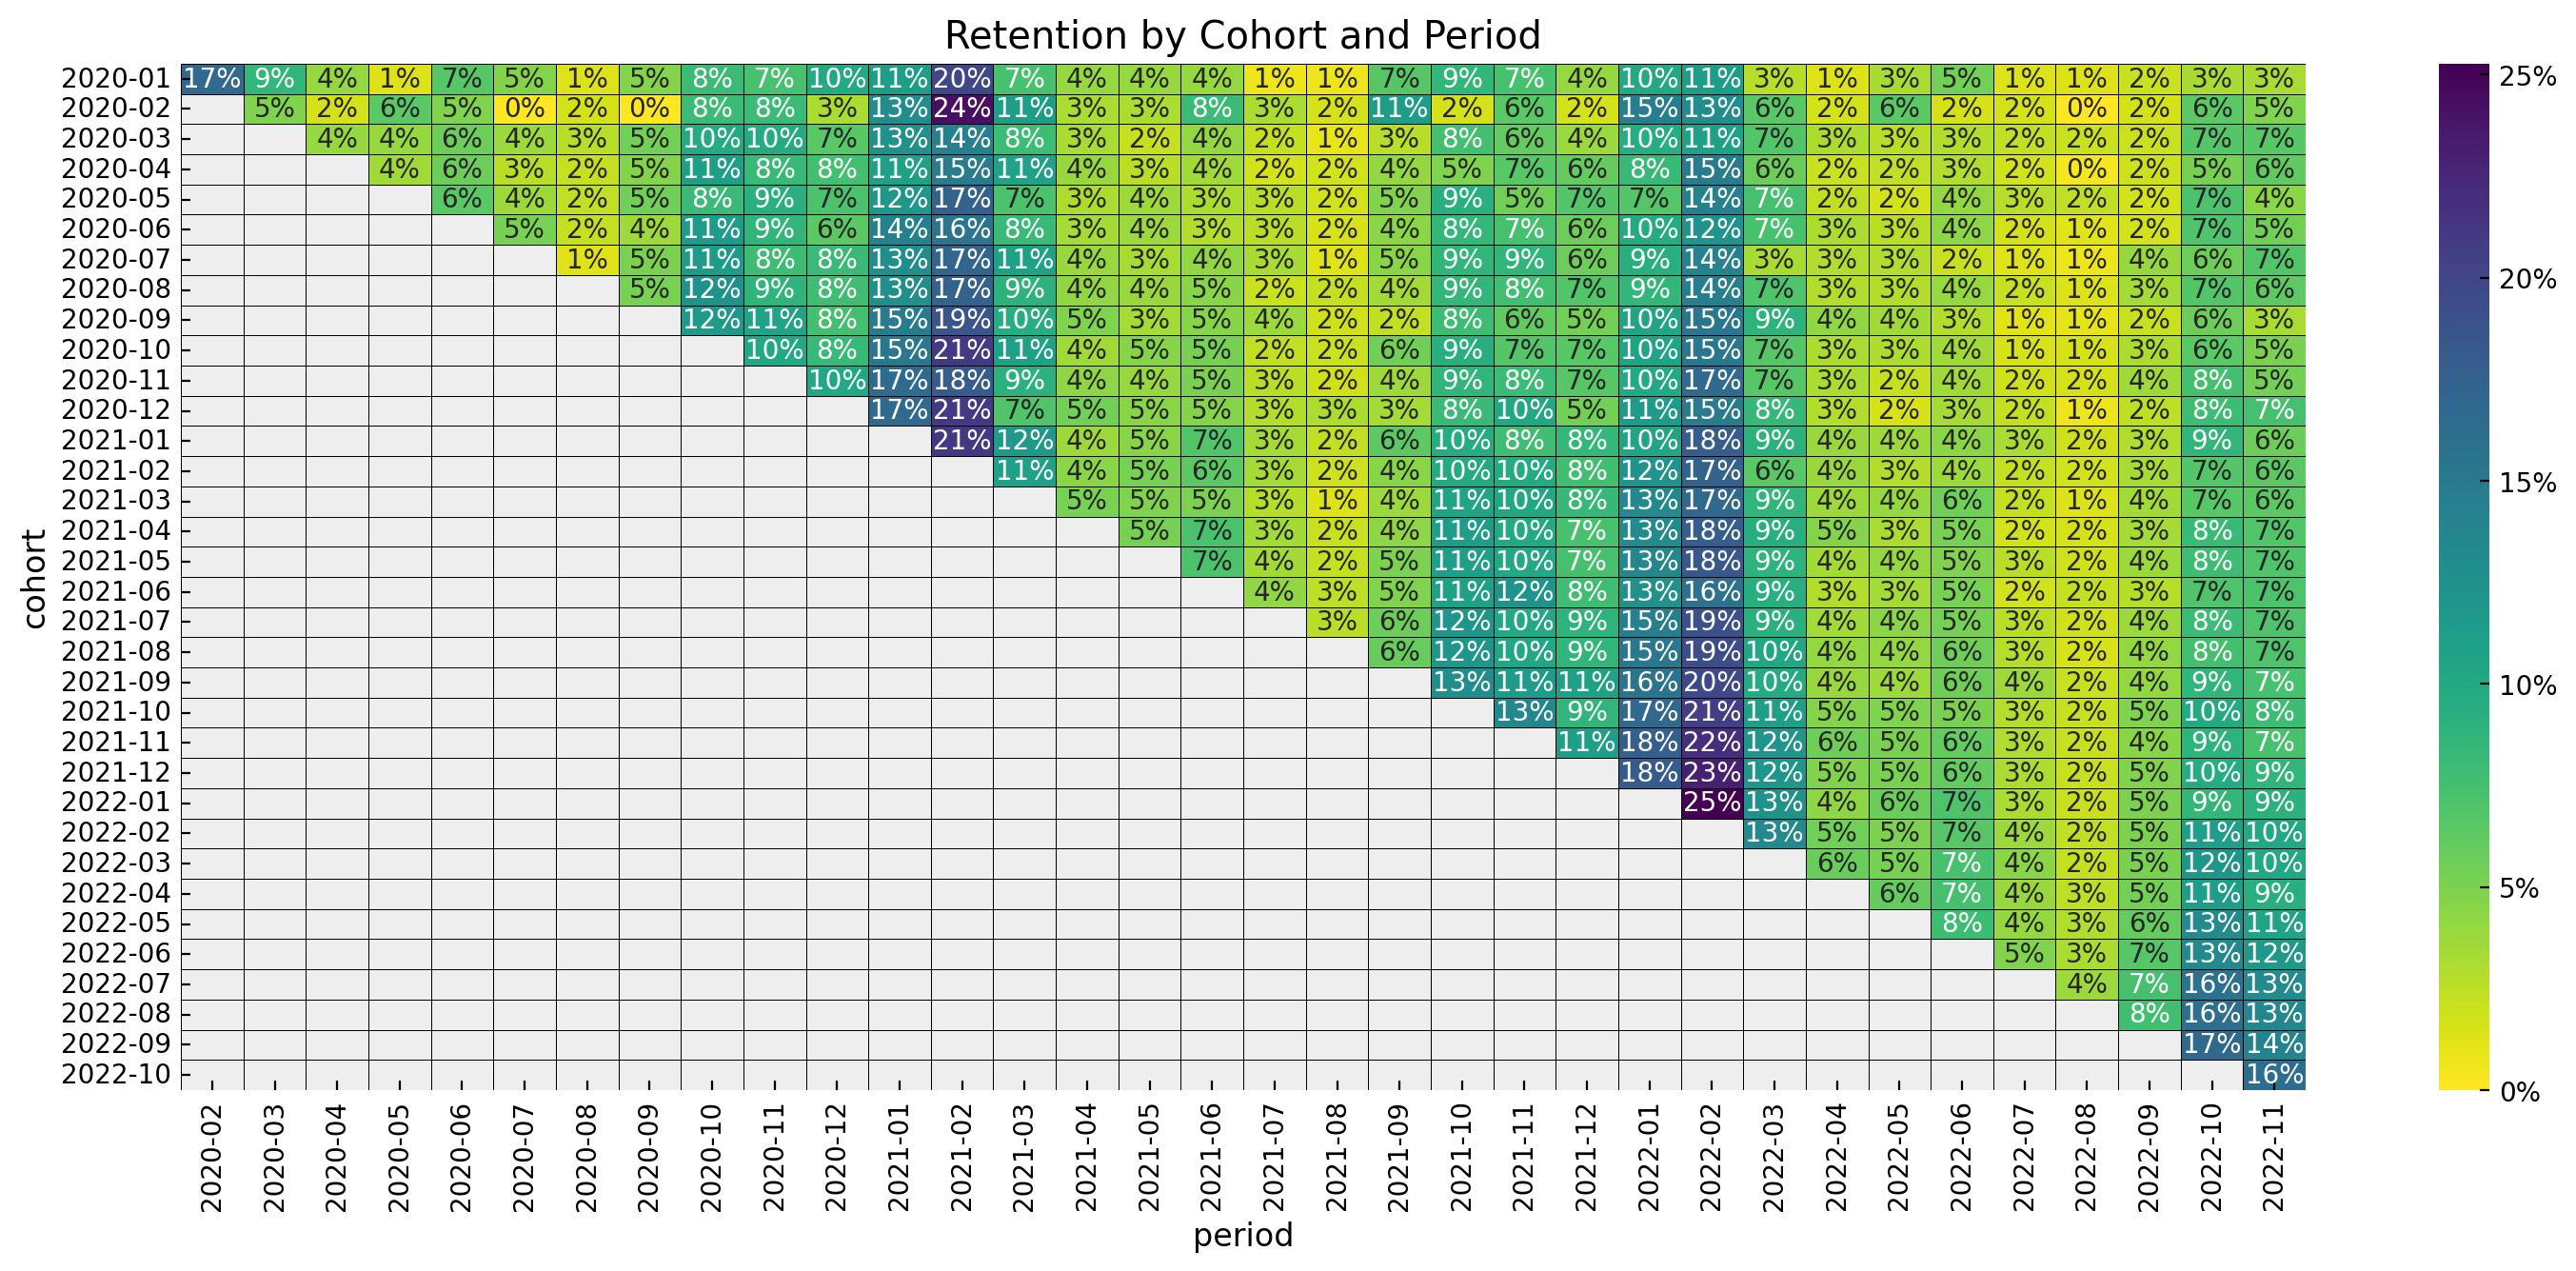
\includegraphics[width=\textwidth]{images/revenue_retention_17_0.png}

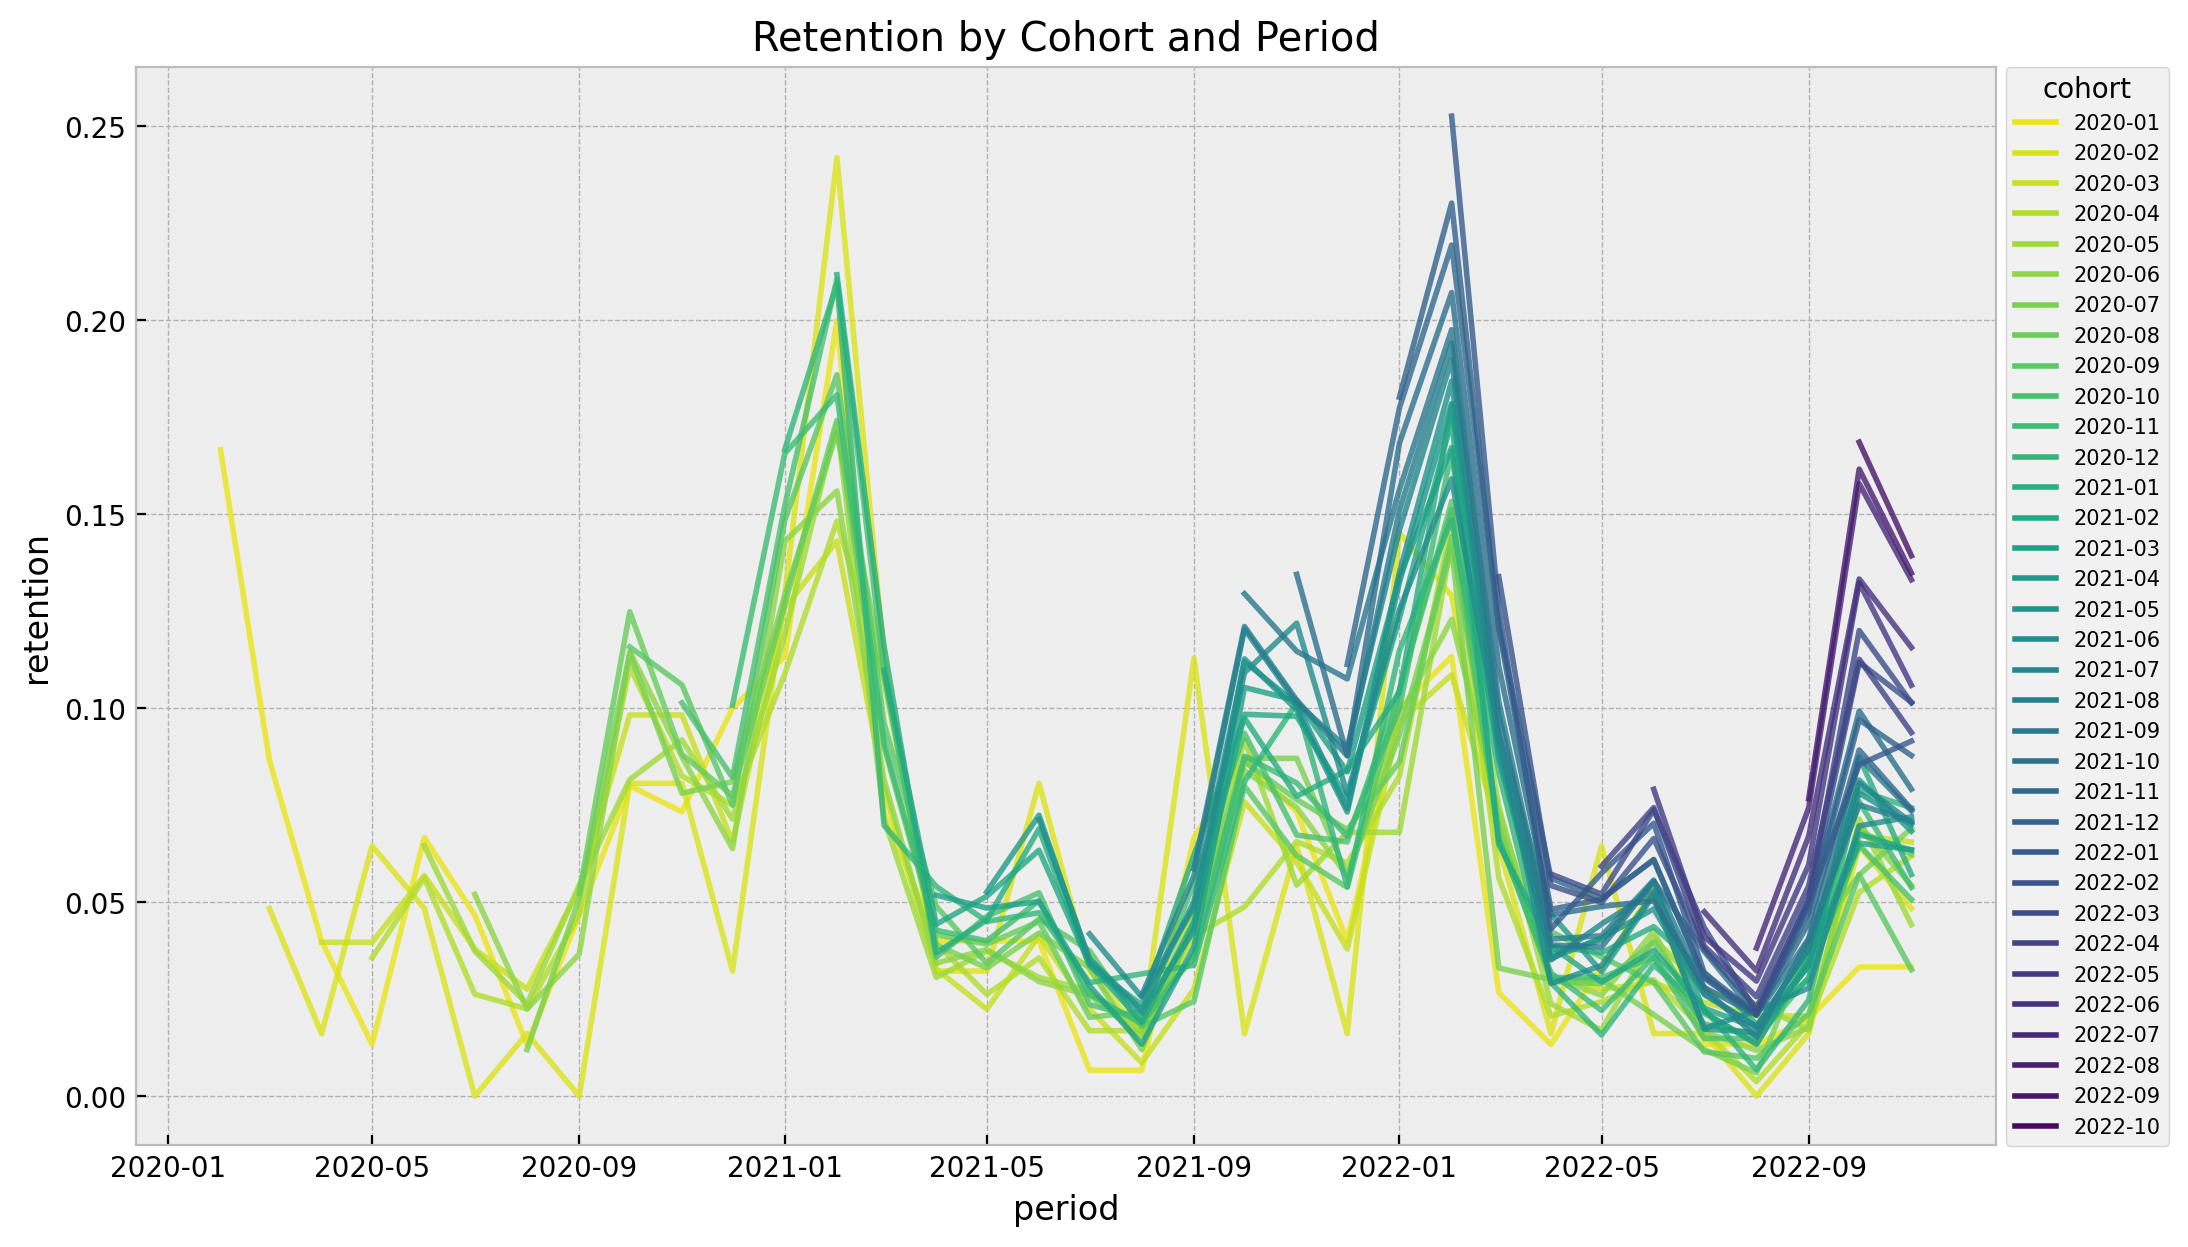
\includegraphics[width=\textwidth]{images/revenue_retention_19_0.png}

\appendix{Appendix: Python Code}

\begin{lstlisting}[language=Python, caption=Python example]
import pymc_bart as pmb
import pymc as pm


with pm.Model(coords={"feature": features}) as model:

    # --- Data ---
    model.add_coord(name="obs", values=train_obs_idx, mutable=True)
    age_scaled = pm.MutableData(
        name="age_scaled", value=train_age_scaled, dims="obs"
    )
    cohort_age_scaled = pm.MutableData(
        name="cohort_age_scaled", value=train_cohort_age_scaled, dims="obs"
    )
    x = pm.MutableData(name="x", value=x_train, dims=("obs", "feature"))
    n_users = pm.MutableData(name="n_users", value=train_n_users, dims="obs")
    n_active_users = pm.MutableData(
        name="n_active_users", value=train_n_active_users, dims="obs"
    )
    revenue = pm.MutableData(name="revenue", value=train_revenue, dims="obs")

    # --- Priors ---
    intercept = pm.Normal(name="intercept", mu=0, sigma=1)
    b_age_scaled = pm.Normal(name="b_age_scaled", mu=0, sigma=1)
    b_cohort_age_scaled = pm.Normal(name="b_cohort_age_scaled", mu=0, sigma=1)
    b_age_cohort_age_interaction = pm.Normal(
        name="b_age_cohort_age_interaction", mu=0, sigma=1
    )

    # --- Parametrization ---
    # The BART component models the image of the retention rate under the
    # logit transform so that the range is not constrained to [0, 1].
    mu = pmb.BART(name="mu", X=x, Y=train_retention_logit, m=50, dims="obs")
    # We use the inverse logit transform to get the retention rate
    # back into [0, 1].
    p = pm.Deterministic(name="p", var=pm.math.invlogit(mu), dims="obs")
    # We add a small epsilon to avoid numerical issues.
    p = pt.switch(pt.eq(p, 0), eps, p)
    p = pt.switch(pt.eq(p, 1), 1 - eps, p)

    # For the revenue component we use a Gamma distribution where we
    # combine the number of estimated active users with the average
    # revenue per user.
    lam_log = pm.Deterministic(
        name="lam_log",
        var=intercept
        + b_age_scaled * age_scaled
        + b_cohort_age_scaled * cohort_age_scaled
        + b_age_cohort_age_interaction * age_scaled * cohort_age_scaled,
        dims="obs",
    )

    lam = pm.Deterministic(name="lam", var=pm.math.exp(lam_log), dims="obs")

    # --- Likelihood ---
    n_active_users_estimated = pm.Binomial(
        name="n_active_users_estimated",
        n=n_users,
        p=p,
        observed=n_active_users,
        dims="obs",
    )

    x = pm.Gamma(
        name="revenue_estimated",
        alpha=n_active_users_estimated + eps,
        beta=lam,
        observed=revenue,
        dims="obs",
    )

    # --- Derived Quantities ---
    mean_revenue_per_user = pm.Deterministic(
        name="mean_revenue_per_user", var=(1 / lam), dims="obs"
    )
    pm.Deterministic(
        name="mean_revenue_per_active_user",
        var=p * mean_revenue_per_user,
        dims="obs"
    )
\end{lstlisting}

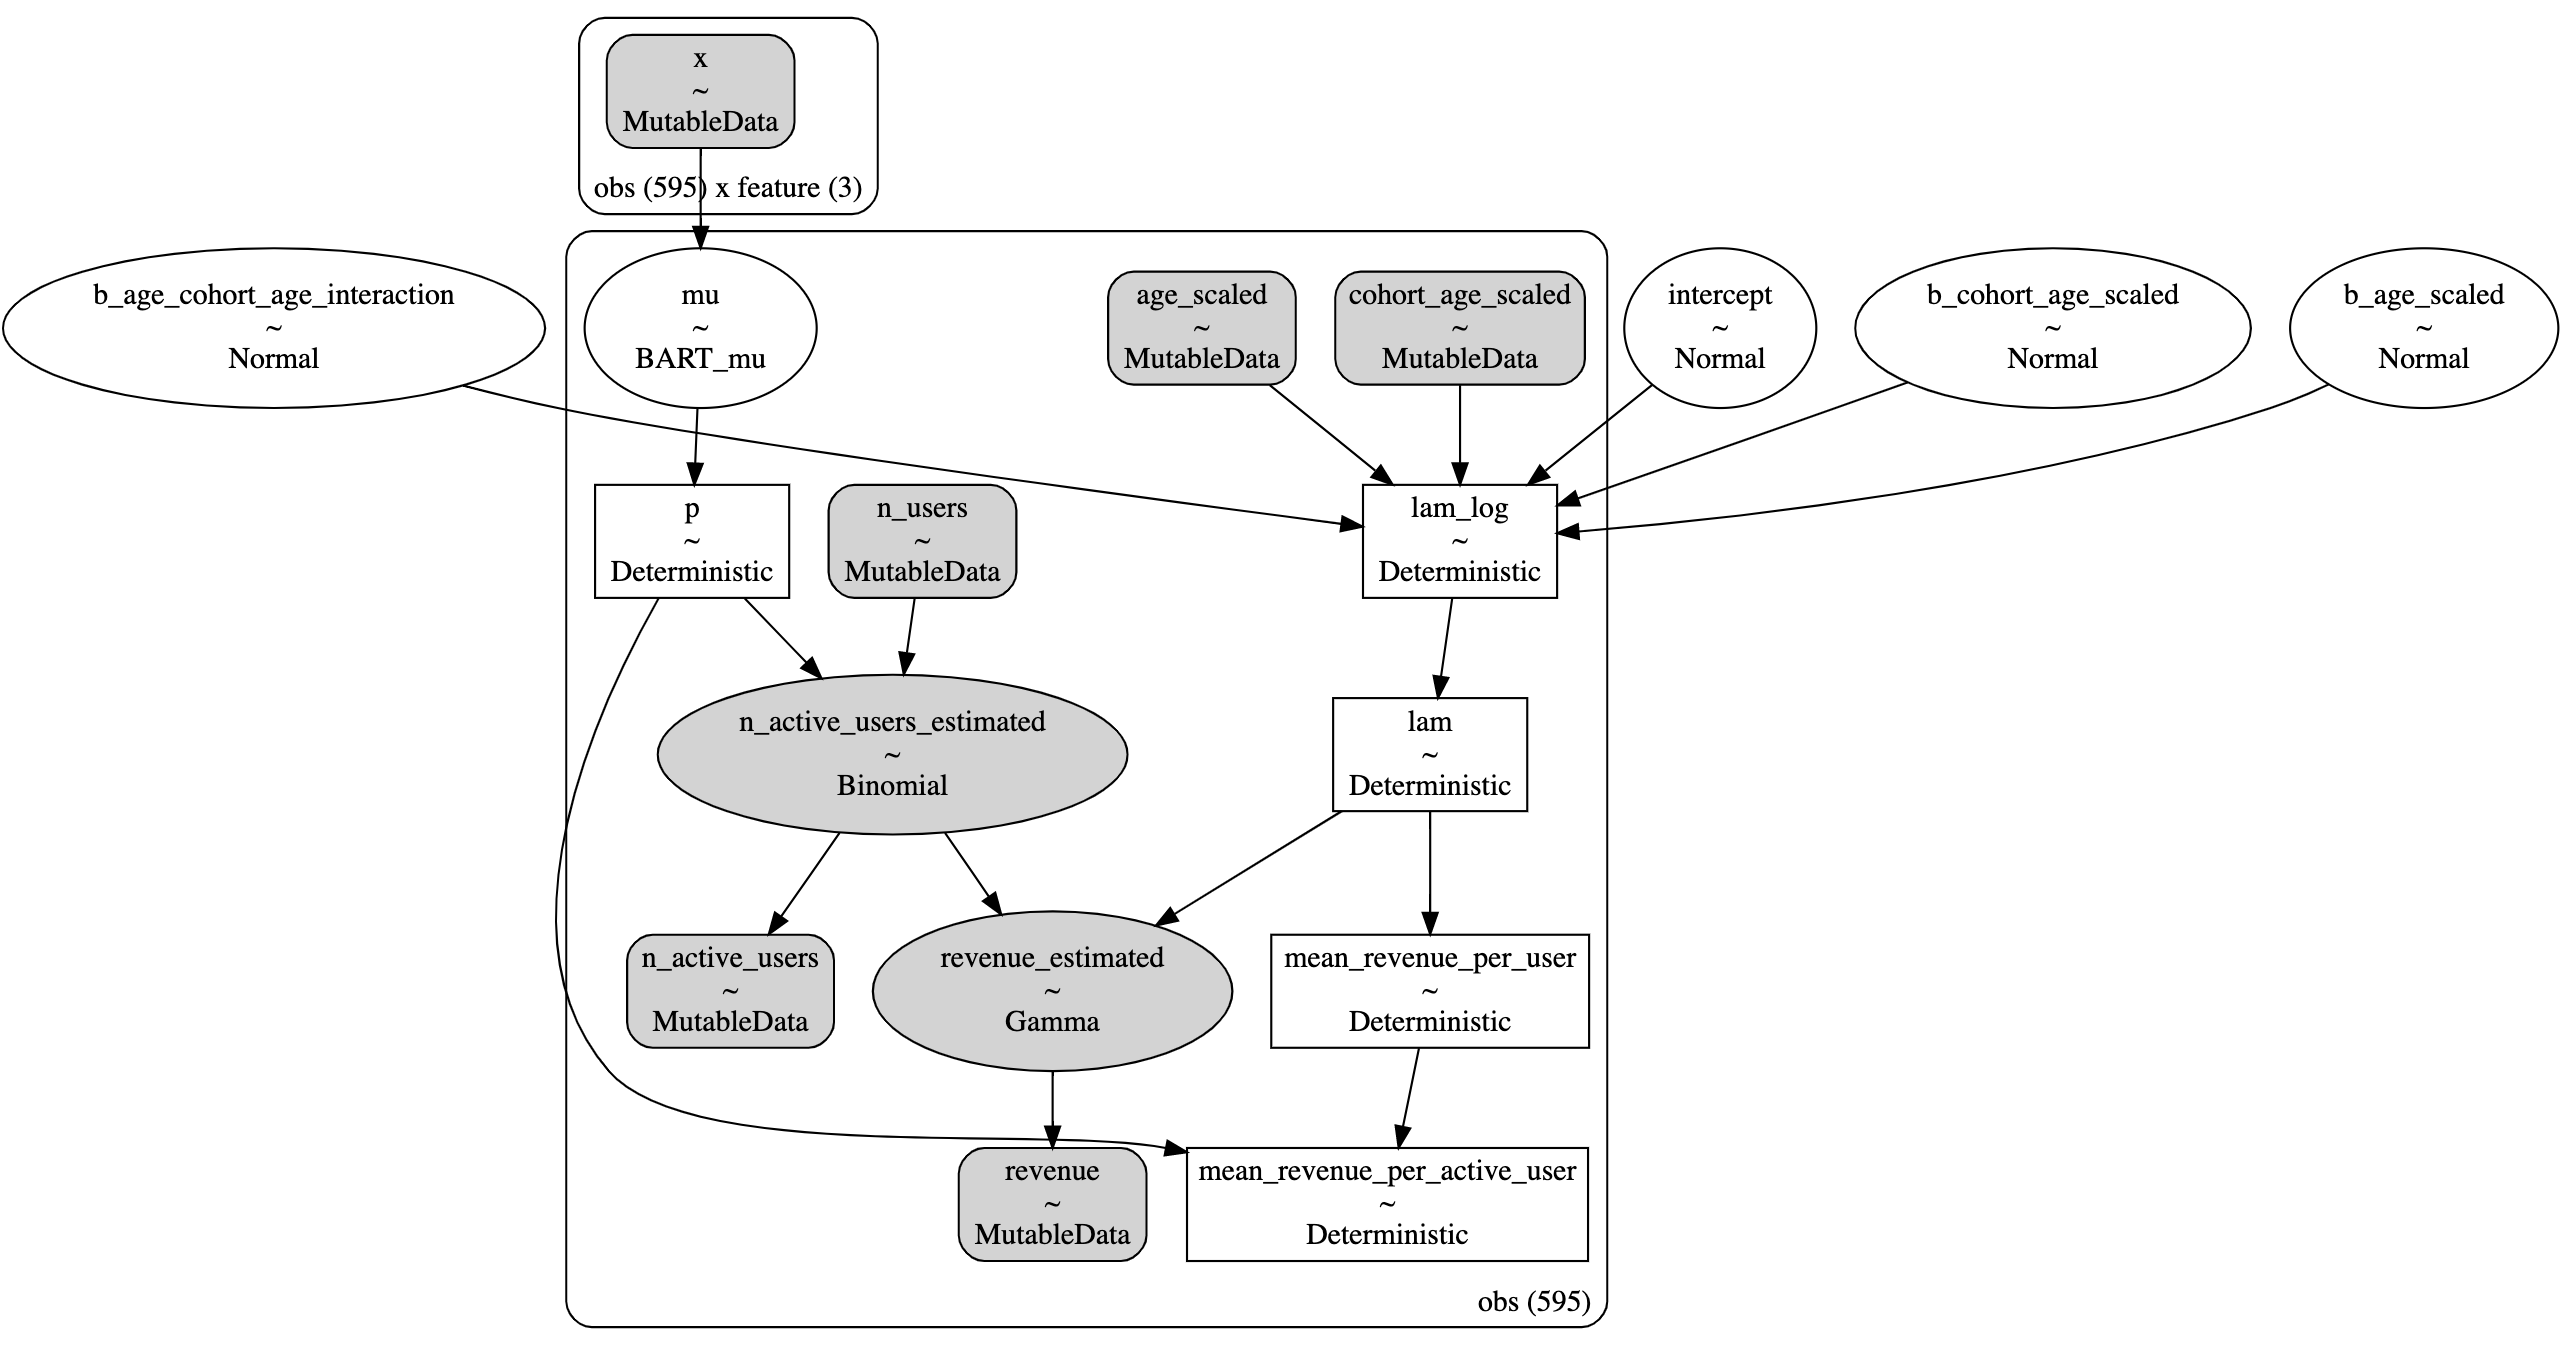
\includegraphics[width=\textwidth]{images/revenue_retention_33_0.png}


\end{document}